% !TEX encoding = UTF-8 Unicode

% !TEX root = ObiStein.tex

%%---------------------
%\title{Estelas en el mar: recordando a Ireneo Peral}
%\author{David Arcoya, Jes\'us Garc\'ia Azorero, Ana Primo y Fernando Soria}
%%---------------------
%
%%---------------------
%\contact{David Arcoya, Dpto. de Matem\'aticas, Universidad de Granada}
%{darcoya@ugr.es}{}
%\contact{Jes\'us Garc\'{\i}a Azorero, Dpto. de Matem\'aticas, Universidad Aut\'onoma de Madrid}
%{jesus.azorero@uam.es}{}
%\contact{Ana Primo, Dpto. de Matem\'aticas, Universidad Aut\'onoma de Madrid}
%{ana.primo@uam.es}{}
%\contact{Fernando Soria, Dpto. de Matem\'aticas, Universidad Aut\'onoma de Madrid}
%{fernando.soria@uam.es}{}
%%---------------------
%
%%---------------------
%\makesemititle
%%---------------------

%Paco
\subsection{Estelas en el mar: recordando a Ireneo Peral (1946--2021)}

\begin{center}\large
\textbf{David Arcoya}$^1$, \textbf{Jes\'us Garc\'ia Azorero}$^2$,\\ \textbf{Ana Primo}$^2$ y
\textbf{Fernando Soria}$^2$\\[1em]
$^1$Universidad de Granada,\\ $^2$Universidad Aut\'onoma de Madrid,\\ 
{\color{azulsema}\rule{.5\linewidth}{1pt}}
\end{center}
%

<<Estelas en el mar>>. Con ese nombre titul\'o Ireneo Peral su conferencia de clausura del congreso internacional {\it New trends in Partial Differential Equations} celebrado en Granada en mayo de 2017. Pod\'ia haber hablado de muchas cosas. Despu\'es de todo, el congreso se celebraba en su honor por su 70 cumplea\~nos y, por tanto, por su inminente jubilaci\'on. Habl\'o de matem\'aticas, por supuesto, y por una vez nos habl\'o tambi\'en de \'el, de sus proyectos, de c\'omo hab\'ia sido su vida hasta entonces y, sobre todo, de sus grandes pasiones: su familia, sus amigos, el trabajo. Ireneo falleci\'o el pasado 16 de febrero y reproducir aqu\'i lo que entonces nos cont\'o ser\'ia la mejor forma de recordarlo, el mejor homenaje que ofrecerle. Pero esa es una tarea imposible y solo nos queda la opci\'on de hacer un recuento, quiz\'as de una forma desordenada, de lo que su vida y su obra han supuesto para aquellos que tuvimos la suerte de conocerlo.

\begin{figure}[h]
\begin{center}
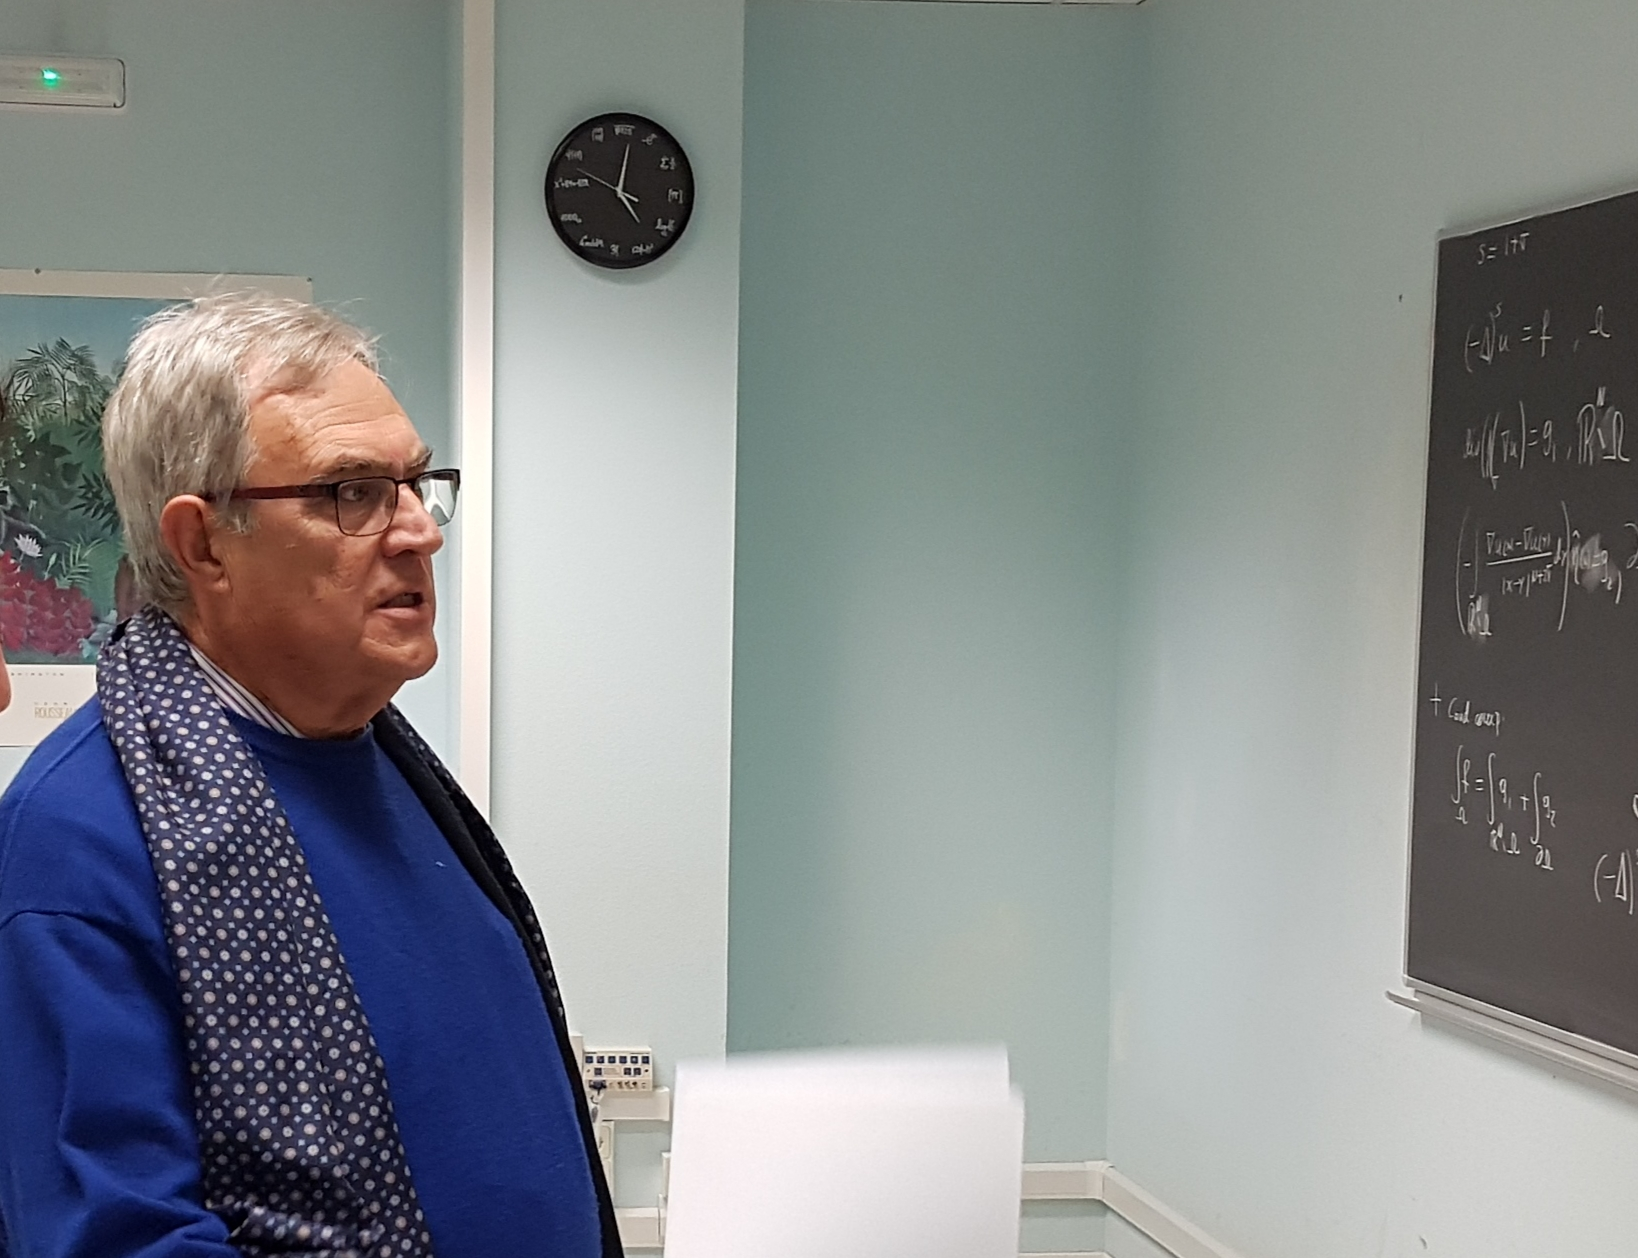
\includegraphics[width=0.7\linewidth]{IP_foto_UAM.jpg}
\caption{Ireneo trabajando en la UAM.}
\end{center}
\end{figure}

En la p\'agina web personal de Ireneo de la Universidad Aut\'onoma de Madrid se puede leer un poema de Borges,  {\it  Los Justos}.  Dice as\'i:

\begin{quote}
\textit{
Un hombre que cultiva su jard\'in, como quer\'ia Voltaire./
    El que agradece que en la tierra haya m\'usica./
    El que descubre con placer una etimolog\'ia./
    Dos empleados que en un caf\'e del Sur juegan un silencioso ajedrez./
    El ceramista que premedita un color y una forma./
    Un tip\'ografo que compone bien esta p\'agina, que tal vez no le agrada./
    Una mujer y un hombre que leen los tercetos finales de cierto canto./
    El que acaricia a un animal dormido./
    El que justifica o quiere justificar un mal que le han hecho./
    El que agradece que en la tierra haya Stevenson./
    El que prefiere que los otros tengan raz\'on./
    Esas personas, que se ignoran, est\'an salvando el mundo.
  }
 \end{quote}



Ireneo era una persona sensible y seguro que estos versos le ayudaban a expresar mejor el sentido de la vida tal como \'el la percib\'ia. Su car\'acter le hac\'ia ser optimista por naturaleza, alguien que busca la felicidad, la suya y, a ser posible, la de los que le rodean.    En una de las transparencias de su charla en Granada nos mostr\'o a modo de dec\'alogo lo que para \'el significaban las Matem\'aticas desde un punto de vista muy personal. De forma breve, dec\'ia lo siguiente: 
\begin{itemize}
\item Las Matem\'aticas son un magn\'ifico reto intelectual.
\item Considero un privilegio trabajar en Matem\'aticas, porque disfruto con ellas.
\item Las Matem\'aticas son una ciencia experimental [!`y a los hechos me remito!]
\item Me veo a mi mismo como un estudiante inexperto al que le gusta ir m\'as all\'a de lo que se conoce, buscando nuevos problemas <<en el lado oscuro>> \,de la ciencia.
\item Odio la tristeza en nuestro trabajo \dots
\end{itemize}

\begin{figure}%[h]
\begin{center}
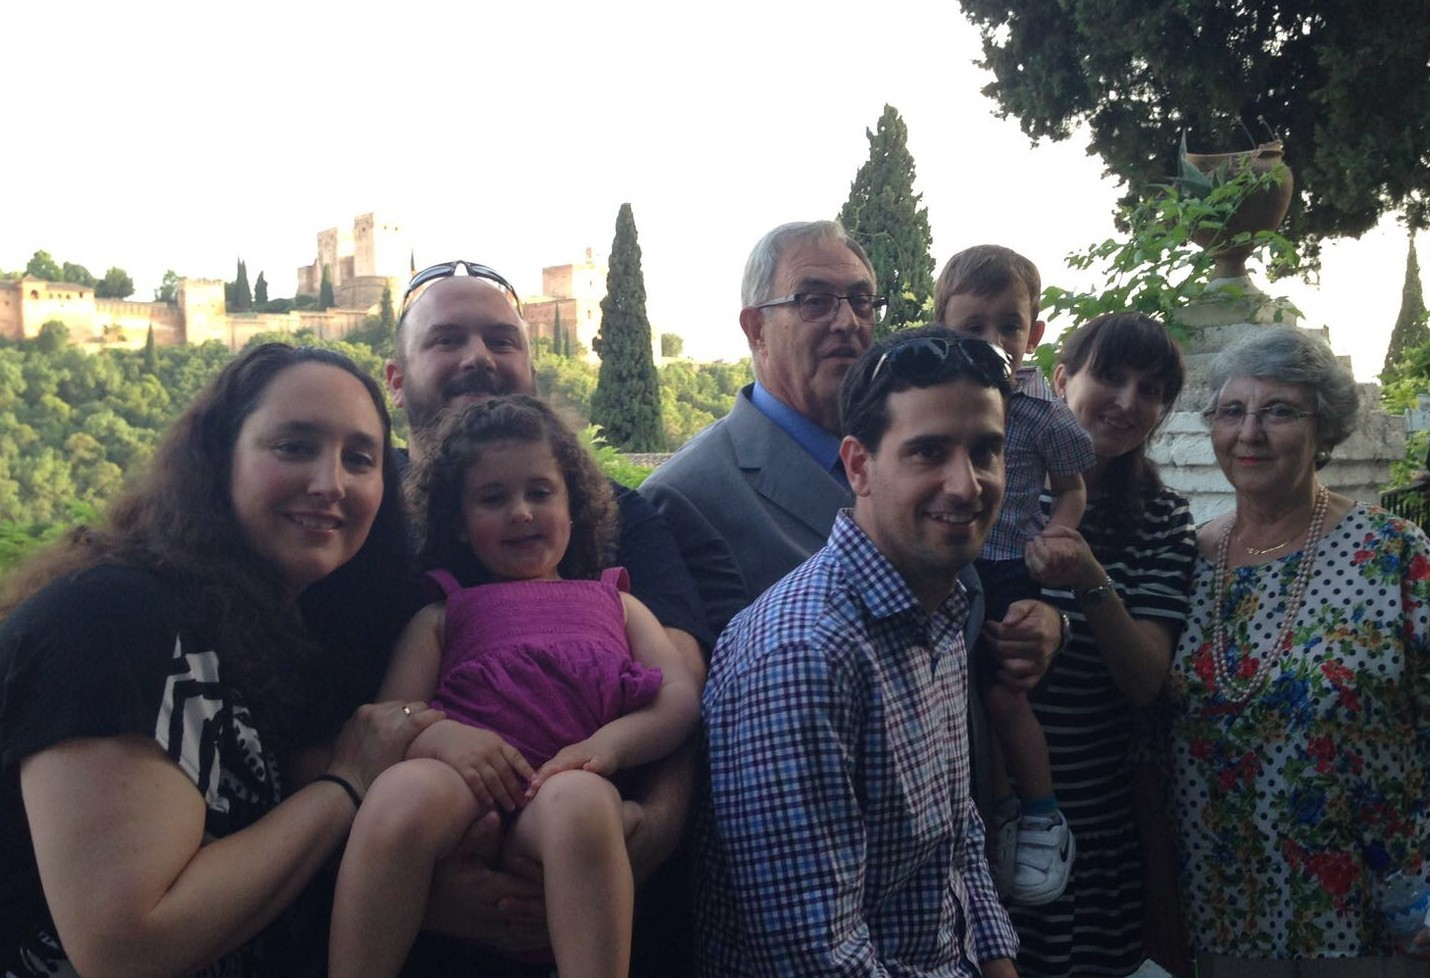
\includegraphics[width=0.9\linewidth]{IP_foto_granada1.jpg}
\caption{Ireneo y Magdalena a los pies de la Alhambra en 2017, con sus hijas, Irene y Magdalena, yernos, David y Carlos, y nietos, Iria y \'Oscar.}
\end{center}
\end{figure}

 
    
Optimismo -y buen humor- son solo algunos de los rasgos que mejor describen a Ireneo. Pero hay muchos otros, como humildad, sencillez,  generosidad y, muy especialmente, el sentido del agradecimiento, que van unidos a su persona. Consideraba que la relaci\'on humana se debe cimentar necesariamente en ser agradecido . Y as\'i lo hizo mencionando a sus padres, a sus hermanos, a su esposa y compa\~nera de tant\'isimos a\~nos, Magdalena Walias,
a sus hijas, a sus nietos y a sus colegas. En otro de los puntos sobre su visi\'on personal de las Matem\'aticas que mencion\'o en la ya citada charla de Granada en 2017, Ireneo escribe:

\begin{quote}
\textit{Creo que he sido muy afortunado de haber conocido a matem\'aticos del m\'as alto nivel humano y cient\'ifico, que me han ense\~nado a trabajar. Entre ellos quiero mencionar a cuatro de ellos que me han ayudado directamente en mi vida profesional: Antonio Ambrosetti, Lucio Boccardo, Luis Caffarelli  e Yves Meyer.}
\end{quote}

Esta misma referencia a los que \'el llam\'o m\'as tarde mis <<maestros>>\footnote{Ireneo puede considerarse un autodidacta en muchos aspectos, especialmente en el origen de su trabajo en EDP. Creemos que esto es compatible no obstante con la profunda convicci\'on que \'el siempre tuvo sobre el papel que jugaron estas personas   en su trayectoria  cient\'ifica y con las que  mantuvo una relaci\'on de amistad muy entra\~nable. V\'ease, por ejemplo,  la entrevista que Ireneo realiz\'o a Yves Meyer para {\sc La Gaceta}  con ocasi\'on de la entrega a este del premio Abel en 2017  (\cite{IP1}).} aparece en el pr\'ologo del libro que estaba terminando de corregir cuando la enfermedad le sorprendi\'o {(\cite{PSbook})}. Quer\'ia poner a todos los que le hab\'ian ayudado de una forma u otra y sufr\'ia con la idea de olvidarse de alguien. En este art\'iculo hemos querido dar la palabra a sus maestros para que nos hablen de sus recuerdos sobre Ireneo. Esta nota concluye con las rese\~nas de cada uno de ellos. Desgraciadamente, Antonio Ambrosetti falleci\'o en noviembre de 2020 y no podr\'a participar en este homenaje. Ambos colaboraron en numerosos trabajos de investigaci\'on, en la organizaci\'on de congresos y escuelas de verano, compartieron estudiantes e, incluso, Antonio Ambrosetti fue nombrado \textit{Doctor honoris causa} por la Universidad Aut\'onoma de Madrid, siendo Ireneo su padrino.  Su profunda amistad rebasaba los l\'imites acad\'emicos. Era entra\~nable escuchar sus charlas futbol\'isticas o culinarias. Las familias de ambos manten\'ian una estrecha relaci\'on que, a pesar de su ausencia, persiste a\'un hoy en d\'ia. A la muerte de Antonio, fue Ireneo, junto con David Arcoya, el encargado de elaborar la rese\~na publicada en {\sc La Gaceta}  para recordar su figura (\cite{AP}).



Tambi\'en hemos pedido a su familia, en la figura de su hermano Juan Carlos, que nos de una visi\'on m\'as cercana de nuestro querido Ireneo. A todos ellos les damos las gracias por su generosidad al aceptar la petici\'on que les  hemos hecho llegar y unimos sus escritos a este homenaje que nunca nos hubiera gustado hacer de forma tan temprana.

\subsection*{Obra cient\'ifica}

La tesis doctoral de Ireneo, defendida en 1974, vers\'o sobre la Teor\'ia de Diferenciaci\'on de Integrales, una incipiente \'area del An\'alisis  que hab\'ia llegado a Espa\~na de la mano de su director, Miguel de Guzm\'an. Este  a su vez hab\'ia sido estudiante de Alberto Calder\'on, uno de los fundadores, junto a Antoni Zygmund,  de la llamada Escuela de An\'alisis de Chicago. Adem\'as de publicar varios art\'iculos que relacionaban convergencia con acotaciones d\'ebiles del operador maximal asociado, Ireneo fue el co-organizador de los dos primeros congresos de An\'alisis Arm\'onico de El Escorial que, de forma ininterrumpida, se vienen celebrando desde entonces cada cuatro a\~nos en este lugar de la sierra de Madrid. El primero lo organiz\'o conjuntamente con Miguel de Guzm\'an, el segundo con Jos\'e Luis Rubio de Francia. Esta faceta como analista arm\'onico dur\'o poco porque enseguida su atenci\'on gir\'o hacia el mundo de la ecuaciones en derivadas parciales no lineales. Sin embargo, en muchos de sus art\'iculos posteriores se puede apreciar su manejo  en esa \'area, especialmente a la hora de utilizar argumentos de tipo geom\'etrico, como los lemas de cubrimiento o la descomposici\'on de Calder\'on-Zygmund.

A lo largo de su dilatada carrera, Ireneo se interes\'o por muchos temas distintos dentro de la ecuaciones en derivadas parciales no lineales. Se sent\'ia especialmente orgulloso de sus resultados en problemas relacionados con el potencial de Hardy; de hecho, como ya se ha mencionado anteriormente, la enfermedad le sorprendi\'o mientras terminaba de corregir las pruebas de imprenta de su  libro sobre este tema, \textit{Elliptic  and Parabolic Equations Involving the Hardy-Leray Potential} (\cite{PSbook}). 
El libro, escrito conjuntamente con Fernando Soria,  recoge una gran parte de su obra. Fue terminado de corregir y publicado a principios de 2021.

Pero antes de llegar al potencial de Hardy, hubo mucho trabajo previo. Por ejemplo, Ireneo siempre record\'o con especial cari\~no un trabajo con Juli\'an Aguirre, sobre soluciones peri\'odicas para la ecuaci\'on de ondas {(ver \cite{Aguirre-Peral})}. Luego, en 1985, se embarc\'o en la direcci\'on de la tesis doctoral de Jes\'us Garc\'ia Azorero. Y, como siempre, lo hizo de forma entusiasta, proponiendo problemas, proporcionando referencias y ayudando con una gu\'ia constante y eficaz. El objetivo inicial fue conseguir una cierta soltura con los m\'etodos variacionales a trav\'es de un operador que entonces empezaba a estar de moda, el $p$-laplaciano, definido por 
$$ -\Delta_p u= -\hbox{div}(|\nabla u|^{p-2} \nabla u).$$ 
As\'i, al salir del caso lineal $p=2$ hab\'ia un gran campo por explorar. En particular, todo lo relacionado con los problemas que inclu\'ian el exponente cr\'itico de Sobolev, siguiendo los pasos del c\'elebre trabajo de {Brezis-Nirenberg} para el caso del laplaciano cl\'asico. El problema era c\'omo conseguir la condici\'on de compacidad de Palais-Smale local en el caso no lineal.  Una de las caracter\'isticas de Ireneo era siempre su amplia cultura matem\'atica y su conocimiento de los \'ultimos avances. Por aquel tiempo, aparecieron publicados en la reci\'en nacida \textit{Revista Matem\'atica Iberoamericana}
 dos excelentes art\'iculos de {Pierre Louis Lions} en los que daba una versi\'on muy clara y detallada del principio de concentraci\'on-compacidad. Entender estos art\'iculos fue la clave para poder demostrar la deseada condici\'on de compacidad y obtener los  resultados que presentamos a continuaci\'on en los problemas con exponente cr\'itico.

Dado el problema
$$\left\{
\begin{array}{rl}
-\Delta_p u & = \lambda |u|^{q-2} u + |u|^{p^*-2} u, \, \hbox{ en }  \Omega, \\[1mm]
u|_{\partial \Omega} &= 0, 
\end{array}\right.
$$
siendo $\Omega $ un dominio acotado y regular en $ \mathbb{R}^N $, $ p <N $  y $ p^* = {Np}/{(N-p)} $ el exponente cr\'itico de Sobolev, se tienen los resultados siguientes: 
\begin{itemize}
\item Si $ p < q < p^*$, existe una constante positiva $ \lambda_0$ tal que el problema cr\'itico tiene al menos una soluci\'on positiva para todo $ \lambda > \lambda_0$.
\item  Si $\max \{ p, p^*-  p/(p-1)\} <q<p^*$, el problema cr\'itico tiene al menos una soluci\'on positiva para todo $\lambda >0 $.
\item Si $ q=p, \, N\ge p^2 $, el problema cr\'itico tiene al menos una soluci\'on positiva cuando $ 0<\lambda< \lambda_1(p)$ (siendo $\lambda_1(p)$ el primer autovalor del $p$-laplaciano en el dominio $ \Omega$). 
\end{itemize}

Estos resultados generalizaban  lo demostrado por {Brezis-Nirenberg} en el caso lineal  $ p=2$. Pero, viendo el rango de par\'ametros, resultaba natural plantearse un caso m\'as: el problema cr\'itico cuando el t\'ermino de perturbaci\'on satisface $ 1<q<p$. Es decir, el equivalente a a\~nadir una potencia {\it c\'oncava } en el caso lineal. En este caso, mediante un sencillo truncamiento, se pudo probar que para valores peque\~nos de $ \lambda $ el t\'ermino dominante era lo que inicialmente se ve\'ia como un t\'ermino de perturbaci\'on, y era posible aplicar la teor\'ia minimax para demostrar la existencia de infinitas soluciones (una de ellas positiva),  todas con energ\'ia negativa.
\begin{itemize}
\item Si $ 1 < q < p$, existe una constante positiva $ \lambda_*$ tal que si $ 0<\lambda <  \lambda_*$ el problema cr\'itico tiene infinitas soluciones. 
\end{itemize}
Este resultado de multiplicidad de soluciones en un problema cr\'itico era interesante, pero claramente mejorable: dejaba la puerta abierta al estudio de la existencia de soluciones con energ\'ia positiva. En cualquier caso, junto con otros resultados (por ejemplo, la prueba del comportamiento asint\'otico de la sucesi\'on de autovalores del $p$-laplaciano obtenidos a partir de la teor\'ias de Lusternink-Schnirelman, o el estudio de problemas con crecimiento exponencial cuando $p=N$) Ireneo consider\'o que era material suficiente como para dar por conclu\'ida una tesis doctoral, que fue defendida en 1989, con el habitual y comprensible alivio tanto del alumno como del director, y cuyos resultados se recogen en varias publicaciones  {(entre ellas \cite{Azorero-Peral_1,Azorero-Peral_4})}. 

Era bastante evidente que el resultado para el problema cr\'itico con $1<q<p$ a\'un dejaba un amplio margen de mejora  y unos a\~nos despu\'es aparecieron dos avances fundamentales. 
Por un lado,  durante una visita de Lucio Boccardo a Espa\~na  en la primavera de 1991, Ireneo, Lucio y otro de sus amigos, Miguel Escobedo, escribieron el trabajo {\cite{Boccardo-Escobedo-Peral}} donde, v\'{\i}a el  m\'etodo de sub-super soluciones,  probaban para valores peque\~nos del par\'ametro $\lambda>0$ la existencia de soluci\'on positiva incluso en problemas supercr\'iticos.  De otro lado, este resultado fue presentado por Lucio Boccardo en un congreso  celebrado en Erice, Italia y capt\'o  la atenci\'on de A. Ambrosetti, H. Brezis y G. Cerami, quienes, usando un elegante argumento de reducci\'on al absurdo y
sin salirse del caso  $ p=2$, consiguieron demostrar la existencia de una segunda soluci\'on positiva\footnote{\textsc{A. Ambrosetti, H. Brezis, G. Cerami}, Combined Effects of Concave and Convex Nonlinearities in Some Elliptic Problems. \textit{J. Funct. Anal.}  \textbf{122} (1994), no.2, 519--543.} y de paso, acu\~naron el t\'ermino {\it c\'oncavo-convexo} que desde entonces ha pasado a ser la manera habitual de referirse a estos problemas.  

La visita anteriormente rese\~nada de Lucio Boccardo a Madrid  fue tambi\'en el germen de otra relaci\'on importante de Ireneo al ponerle en conocimiento de la existencia de un joven matem\'atico en la Universidad de Granada, David Arcoya, que hab\'ia trabajado en Italia con Antonio Ambrosetti y el propio Boccardo. Ireneo tom\'o nota inmediatamente y, tras cursar una invitaci\'on a David para una visita a la Aut\'onoma, comenz\'o un estrecha relaci\'on de tutelaje del incipiente grupo de Granada-Almer\'ia, facilitando su desarrollo hasta llegar a ser el que  hoy en d\'ia conforman el propio David Arcoya, Jos\'e Carmona, Jos\'e Luis G\'amez, David Ruiz  y Salvador Villegas, junto con sus respectivos estudiantes.



Ciertamente, el mundo c\'oncavo-convexo se revel\'o mucho m\'as rico de lo sospechado inicialmente, y dio lugar a una serie de trabajos que tuvieron una repercusi\'on considerable, al menos si aceptamos como unidad de medida el n\'umero de citas, algo que Ireneo miraba habitualmente con un cierto escepticismo. Siempre dec\'ia que lo importante era valorar los resultados, y no usar los rankings para evitar la fastidiosa tarea de pensar. Pero en paralelo, otros muchos problemas captaron la atenci\'on de Ireneo. En particular, en la tesis de Juan Antonio Aguilar (presentada en 1998), comenzaron a explorar el efecto de la presencia de potenciales singulares en el t\'ermino de reacci\'on, tanto en el caso parab\'olico como en el caso el\'iptico, estudiando ecuaciones del tipo $ u_t - \Delta_p u = \lambda V(x) f(u) $ y sus correspondientes estados estacionarios. Cuando $V(x)=|x|^{-\gamma} $ (y, por supuesto, el dominio donde se plantea la ecuaci\'on es un entorno del origen de coordenadas) descubrieron y analizaron una rica variedad de fen\'omenos, dependiendo de las relaciones entre los par\'ametros caracter\'isticos del problema, $ N, \lambda, \gamma$ y $ p $, y tambi\'en de los diferentes t\'erminos de reacci\'on $ f(u)$. Un trabajo muy completo, a la vez que muy meritorio, que dio lugar a numerosos art\'iculos {(entre ellos \cite{Aguilar-Peral_5})} y que fue realizado mientras Juan Antonio  desempe\~naba con \'exito su vida profesional en la empresa privada, robando horas al sue\~no para estudiar las matem\'aticas que tanto le apasionaban. Ireneo, al igual que todos nosotros,  sinti\'o  profundamente su prematura muerte, en plena juventud.


El trabajo de Ambrosetti-Brezis-Cerami antes citado fue muy influyente para Ireneo, por varios motivos. De un lado, porque intentar la extensi\'on de las pruebas all\'i contenidas al caso $ p \ne 2 $ requer\'ia de unos resultados de regularidad, que obtuvo en colaboraci\'on con otro gran matem\'atico y amigo, Juanjo Manfredi, y con Jes\'us Garc\'ia Azorero {(\cite{Azorero-Manfredi-Peral})}. Pero sobre todo, porque a ra\'iz de la aparici\'on de ese art\'iculo Ireneo invit\'o a Antonio Ambrosetti a visitar el Departamento de Matem\'aticas de la Universidad Aut\'onoma. {Esta primera visita de Antonio tuvo un impacto fundamental en el desarrollo matem\'atico de Ireneo y de todo su grupo de colaboradores, con una producci\'on cient\'ifica conjunta de considerable inter\'es (ve\'anse~[8-12]). Pero sobre todo permiti\'o iniciar una amistad personal sincera y profunda que se mantuvo a lo largo de los a\~nos. Antonio se sent\'ia especialmente c\'omodo con la c\'alida acogida y el ambiente familiar que Ireneo supo crear en su entorno. Esa amistad se tradujo en un contacto permanente y los sucesivos viajes en las dos direcciones permitieron tambi\'en a Ireneo hacerse un hueco importante en los grupos de investigadores italianos, donde era realmente muy querido.}

En aquella \'epoca, el flujo de visitantes en el departamento de matem\'aticas de la Aut\'onoma era constante. En varias etapas tuvo el lujo de acoger como visitante de larga duraci\'on al profesor Grigory Barenblatt. Durante los almuerzos en el comedor de la facultad, Barenblatt era habitualmente el centro de la conversaci\'on. Entre an\'ecdota y an\'ecdota, siempre estaba comentando nuevos modelos, proponiendo cuestiones originales e interesantes. Una de estas conversaciones capt\'o pronto la atenci\'on de Ireneo, que para entonces ya hab\'ia comenzado a leer trabajos relacionados con cuestiones de homogeneizaci\'on: la idea era estudiar un problema de contorno para el laplaciano, u otro operador el\'iptico, con la particularidad de que las condiciones de frontera eran de tipo mixto Dirichlet-Neumann, y el objetivo final era ir moviendo estas condiciones de frontera de una manera uniforme, haciendo que la medida del subconjunto con condici\'on de Dirichlet fuera tendiendo a cero a la velocidad adecuada. Aqu\'i surgieron cuestiones muy interesantes de falta de regularidad, que fueron cuidadosamente estudiadas en la tesis doctoral de Eduardo Colorado, junto con problemas tanto el\'ipticos como parab\'olicos en los que aparec\'ia un operador singular, $ -\Delta_{p,\gamma} u = -\hbox{div}(|x|^{-p\gamma} |\nabla u|^{p-2}\nabla u ) $, relacionado con las desigualdades de Caffarelli-Kohn-Nirenberg (CKN) y reflejado en un  {trabajo inicial} en dicha l\'{\i}nea 
{(\cite{Col-Per2})}. Animado por Ireneo, Eduardo Colorado viaj\'o a Trieste (Italia) a realizar una estancia postdoctoral bajo la direcci\'on de   Antonio Ambrosetti,  hecho que a Ireneo le hizo muy feliz.

Una vez abierta la {\it caja} de los potenciales singulares, inmediatamente se lanz\'o a estudiar los que ser\'ian unos de sus problemas favoritos: los problemas relacionados con el potencial de Hardy. En su reciente libro \cite{PSbook} escribe:
\begin{quote}
\textit{El potencial de Hardy tiene algo fascinante, puede complicar enormemente los c\'alculos pero al mismo tiempo proporciona un conjunto muy rico de propiedades adicionales. En ese sentido es a la vez un monstruo y un amigo.}
\end{quote}
De hecho hay una secci\'on titulada <<D\'onde (y por qu\'e) aparece el monstruo>>,  en la que se explica la importancia de este objeto matem\'atico.

En su primer trabajo en esta \'area, en colaboraci\'on con Jes\'us Garc\'ia Azorero (ver \cite{Azorero-Peral_5}), la idea inicial  fue intentar entender los resultados del c\'elebre trabajo de Baras-Goldstein sobre blow-up instant\'aneo y completo en una ecuaci\'on del calor con t\'ermino de reacci\'on $\lambda \frac u{|x|^2} $ (con $ \lambda>(N-2)/2$), y extenderlos al correspondiente problema con el $p$-laplaciano, donde por cuestiones de homogeneidad el t\'ermino de reacci\'on pasaba a ser $\lambda \frac {u^{p-1}}{|x|^p} $. Una vez m\'as, la presencia del par\'ametro $p$ permiti\'o estudiar fen\'omenos muy interesantes, especialmente en el caso $1<p<2$, en el que para $ \lambda >(N-p)/p$ el blow-up result\'o no ser tan dr\'astico como en el caso lineal, y algunas normas permanec\'ian acotadas. De este modo, se abrieron muchos problemas que requer\'ian nuevas ideas, cuyo estudio recibi\'o el impulso inestimable de la incorporaci\'on de nuevos miembros al grupo de investigaci\'on. As\'i en Noviembre de 1997, lleg\'o Boumediene Abdellaoui a Madrid. Era el  primer estudiante argelino en venir a realizar una tesis de Matem\'aticas a Espa\~{n}a. Se puso en contacto con Ireneo, quien amablemente le recibi\'o (en franc\'es) y le orient\'o acerca de los cursos de doctorado. Tambi\'en le ayud\'o con sus problemas administrativos y le propuso asistir al curso de Jes\'us Garc\'ia Azorero sobre ecuaciones cuasilineales. Al terminar, Boumediene estaba convencido de querer empezar una tesis en Ecuaciones, y volvi\'o a llamar a la puerta de Ireneo para pedirle un problema. Le quedaban solo dos a\~{n}os de beca y <<ten\'ia miedo de no llegar>>, le dijo. Ireneo, con su energ\'ia y entusiasmo caracter\'istico, le contest\'o:  <<ese es el primer signo de que lo conseguir\'as, solo tienes que trabajar>>. Fue el comienzo no solo de una tesis doctoral, sino de una colaboraci\'on muy fruct\'ifera que dio lugar a muy buenos teoremas hasta el final.  Ireneo era el investigador responsable de un proyecto de cooperaci\'on cient\'{\i}fica con Argelia financiado por la Agencia Espa\~nola de Cooperaci\'on Internacional,  y peri\'odicamente se ve\'ian por el Departamento estudiantes argelinos que ven\'ian a aprender con \'el. A d\'ia de hoy, Boumediene Abdellaoui mantiene vivo este legado con la hermosa tarea de formaci\'on de doctores en la Universidad de Tlemcen.

\begin{figure}%[h]
\begin{center}
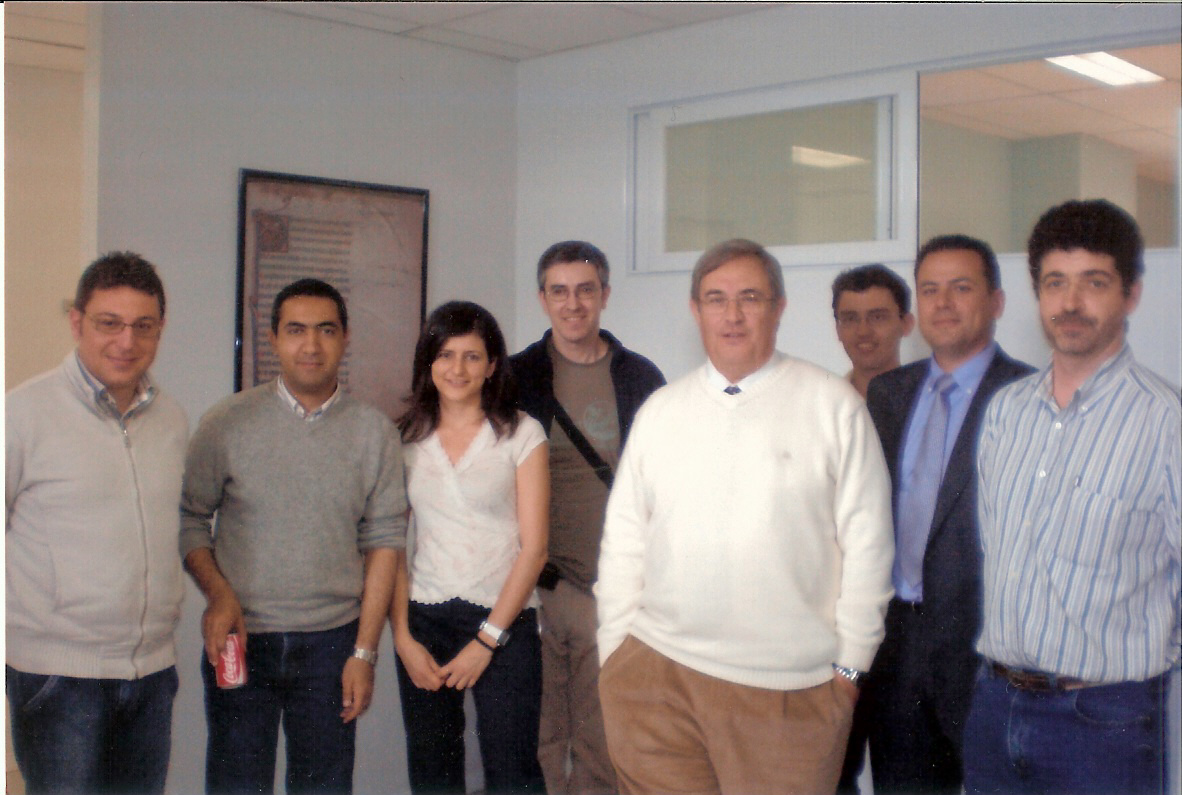
\includegraphics[width=0.9\linewidth]{IP_foto_Alumnos.jpg}
\caption{Ireneo y algunos de sus alumnos de doctorado. De iquierda a derecha, L. Montoro, B. Abdellaoui, A. Primo, E. Colorado, Ireneo, F. Charro, J.A. Aguilar y J. Garc\'ia Azorero.}
\end{center}
\end{figure}


Boumediene comenz\'o a leer el art\'iculo de Brezis-Cabr\'e acerca del potencial de Hardy\footnote{\textsc{H. Brezis, X. Cabr\'e}, Some simple nonlinear PDE's without solutions, \textit{Boll. Unione Mat. Ital.,} \textbf{1} (1998), 223--262.}, con la intenci\'on de extenderlo al $p$-laplaciano. Pero los argumentos usados en el caso lineal, no se aplicaban al caso quasilineal. Ese fue el primer encuentro con la identidad de Picone, una herramienta muy \'util que permiti\'o obtener resultados importantes (tanto para ecuaciones el\'{\i}pticas como parab\'olicas cuasilineales).
 
El objetivo principal de la tesis era estudiar problemas cuasilineales con peso de tipo CKN y t\'erminos singulares. Analizar la existencia o la no existencia de soluciones puede dar lugar a bastantes situaciones sorprendentes dependiendo de la relaci\'on entre el peso y el t\'ermino singular. La filosof\'{\i}a de Ireneo era simple:\\
\centerline{Hardy (universal)+ Harnack (local) $\Rightarrow$ no existencia + Blow-up completo.}\\
Al final, esta idea fue usada en numerosos art\'iculos  {(ver por ejemplo \cite{AP2})}  y estos trabajos dieron lugar a una excelente tesis doctoral.

En Septiembre de 2002, lleg\'o, procedente de la Universidad de Salamanca, otra estudiante para hacer los cursos de doctorado, Ana Primo. De nuevo, Ireneo con su gran capacidad de acogida, se ofreci\'o a ayudarla con el papeleo de la beca FPU del MECD, y tras los cursos de doctorado, le propuso el problema de estudiar la influencia conjunta de un t\'ermino gradiente, tanto en el lado de absorci\'on como de reacci\'on, con el potencial de Hardy:
$$
\left\{\begin{array}{ll}
-\Delta u\pm |\nabla u|^2=\lambda\dfrac{\,u}{|x|^{2}}+ f&\mbox{ en } \Omega,\\
\hspace{2cm}u>0&\mbox{ en } \Omega,\\
\hspace{2cm}u=0&\mbox{ en }\partial\Omega,
\end{array}\right.
$$
con $\Omega\subset\mathbb{R}^N$ un dominio abierto acotado, $\lambda\in \mathbb{R}$, $N\geq 3$, $0\in\Omega$ y $f$ una funci\'on medible positiva.

Por un lado, si el gradiente est\'a en el lado derecho de la ecuaci\'on, 
$$
-\Delta u= |\nabla u|^2+\lambda\dfrac{\,u}{|x|^{2}}+ f\ \mbox{ en } \Omega,\quad u>0\ \mbox{ en }\Omega,\quad u=0\mbox{ en }\ \partial \Omega,
$$
se prob\'o que  para todo $\lambda>0$ no existe soluci\'on, incluso en el sentido m\'as d\'ebil posible. Este hecho muestra fuertemente la influencia del potencial de Hardy, puesto que el problema 
$$
-\Delta u= |\nabla u|^2+ f\ \mbox{ en }\Omega,\quad u>0\ \mbox{ en }\Omega,\quad u=0\ \mbox{ en }\ \partial\Omega,
$$
tiene soluci\'on para un dato adecuado $f$. Adem\'as, si se cambia el potencial de Hardy $|x|^{-2}$ por un peso $g\in L^m(\Omega)$, con 
$m>\frac N2$, y $\lambda_1(g)$ denota el primer autovalor del problema con dicho peso $g$, existe $0<\lambda_0<\lambda_1(g)$ tal que para todo 
$0<\lambda<\lambda_0$, el problema tiene una soluci\'on d\'ebil para un cierto dato $f$. Tambi\'en se prob\'o que la interacci\'on entre el t\'ermino de Hardy y el gradiente produce un blow-up completo. 

Por otro lado, si el gradiente aparece en el lado izquierdo de la ecuaci\'on,
$$
-\Delta u+|\nabla u|^2=\lambda\dfrac{\,u}{|x|^{2}}+ f\ \mbox{ en }\ \Omega,\quad u>0\ \mbox{ en }\ \Omega,\quad u=0\ \mbox{ en }\ \partial \Omega,
$$
se demostr\'o que, si  $\lambda\ge 0$, entonces existe soluci\'on para cada funci\'on $f\in L^1(\Omega)$, $f\geq 0$, {\it sin ninguna restricci\'on en el tama\~{n}o de  $\lambda$}. De hecho, se prob\'o un resultado de existencia para una clase de pesos, los llamados {\it pesos admisibles}. En particular, el potencial de Hardy pertenece a esta clase.  

La importancia de este resultado estaba en el fuerte efecto regularizante del gradiente, ya que en un trabajo de Boccardo, Orsina y Peral {(\cite{BOP})} de 2006 se prueba que para todo $\lambda>0$, la ecuaci\'on 
\begin{equation}
-\Delta u=\lambda\dfrac{u}{|x|^2}+f(x)\quad \mbox{ en }\
\Omega\subset\mathbb{R}^N ,\quad N\ge 3\quad \mbox{ y } \quad 0\in \Omega,
\end{equation}
no tiene en general soluci\'on para una funci\'on positiva $f\in L^1(\Omega)$. A Ireneo le gustaba especialmente este resultado {{(que puede verse en \cite{APP,APP1}).}} En la tesis se estudiaron tambi\'en en profundidad los correspondientes resultados en el mundo parab\'olico {(v\'ease \cite{APP3})}. 

Cuando las cuentas se {\it atascaban}, Ireneo siempre suger\'ia  parar unos d\'ias y cambiar tanto el punto de vista como los argumentos. Cuando no llevaban al resultado esperado, \'el disfrutaba: <<mejor, m\'as interesante, aqu\'i puede haber nuevas ideas. Cuando estudias un problema, tienes que ir viendo el paisaje>>. Ireneo se caracterizaba por ser un empuje para seguir. No hab\'iamos terminado un problema, y ya estaba proponiendo otro. {As\'i ocurri\'o en  2004 durante una visita} de Andrea Dall'Aglio a la UAM. Andrea trabajaba en problemas con dependencia del gradiente y datos generales y dio un seminario en el Departamento, en el que expuso  problemas abiertos en el tema, en particular, habl\'o sobre los c\'alculos radiales de Ferone-Murat para el problema con gradiente cuadrado en la bola: al hacer el cambio de Hopf-Cole, aparece la medida de Dirac en el cero. Con su enorme capacidad de inferir nuevos problemas, Ireneo sugiri\'o pensar qu\'e suceder\'ia con otras medidas, haciendo el cambio al rev\'es. As\'i surgi\'o la idea de clasificar las soluciones poniendo en el lado derecho de la ecuaci\'on medidas singulares con respecto a la capacidad, dando lugar a un resultado de multiplicidad entre Andrea, Ireneo y Boumediene {(\cite{ADP})}.

{Ireneo ten\'ia una mentalidad muy abierta. El mundo de las Matem\'aticas era una gran familia para \'el y siempre insist\'ia a sus estudiantes en discutir con otros matem\'aticos, intercambiar ideas, viajar, trabajar con gente distinta\dots As\'i que, empezando a analizar problemas en esta direcci\'on, surgieron muchas colaboraciones con otros colegas como Magdalena Walias, Daniela Giachetti, Veronica Felli, Lucio Boccardo, Sergio Segura de Le\'on, Alessio Porretta, Anna Mercaldo, Tommaso Leonori  y muchos otros. }


En  2007, se celebr\'o en Salamanca un Congreso homenaje por su 60 cumplea\~{n}os. Ireneo estaba muy contento de que fuera en la ciudad de sus inicios, de la que siempre dec\'ia con cari\~{n}o que la sent\'ia como la Pisa espa\~{n}ola y se lamentaba de no haber impartido all\'i alg\'un curso: <<nadie es profeta en su propia tierra>>, dec\'ia.


\begin{figure}%[h]
\begin{center}
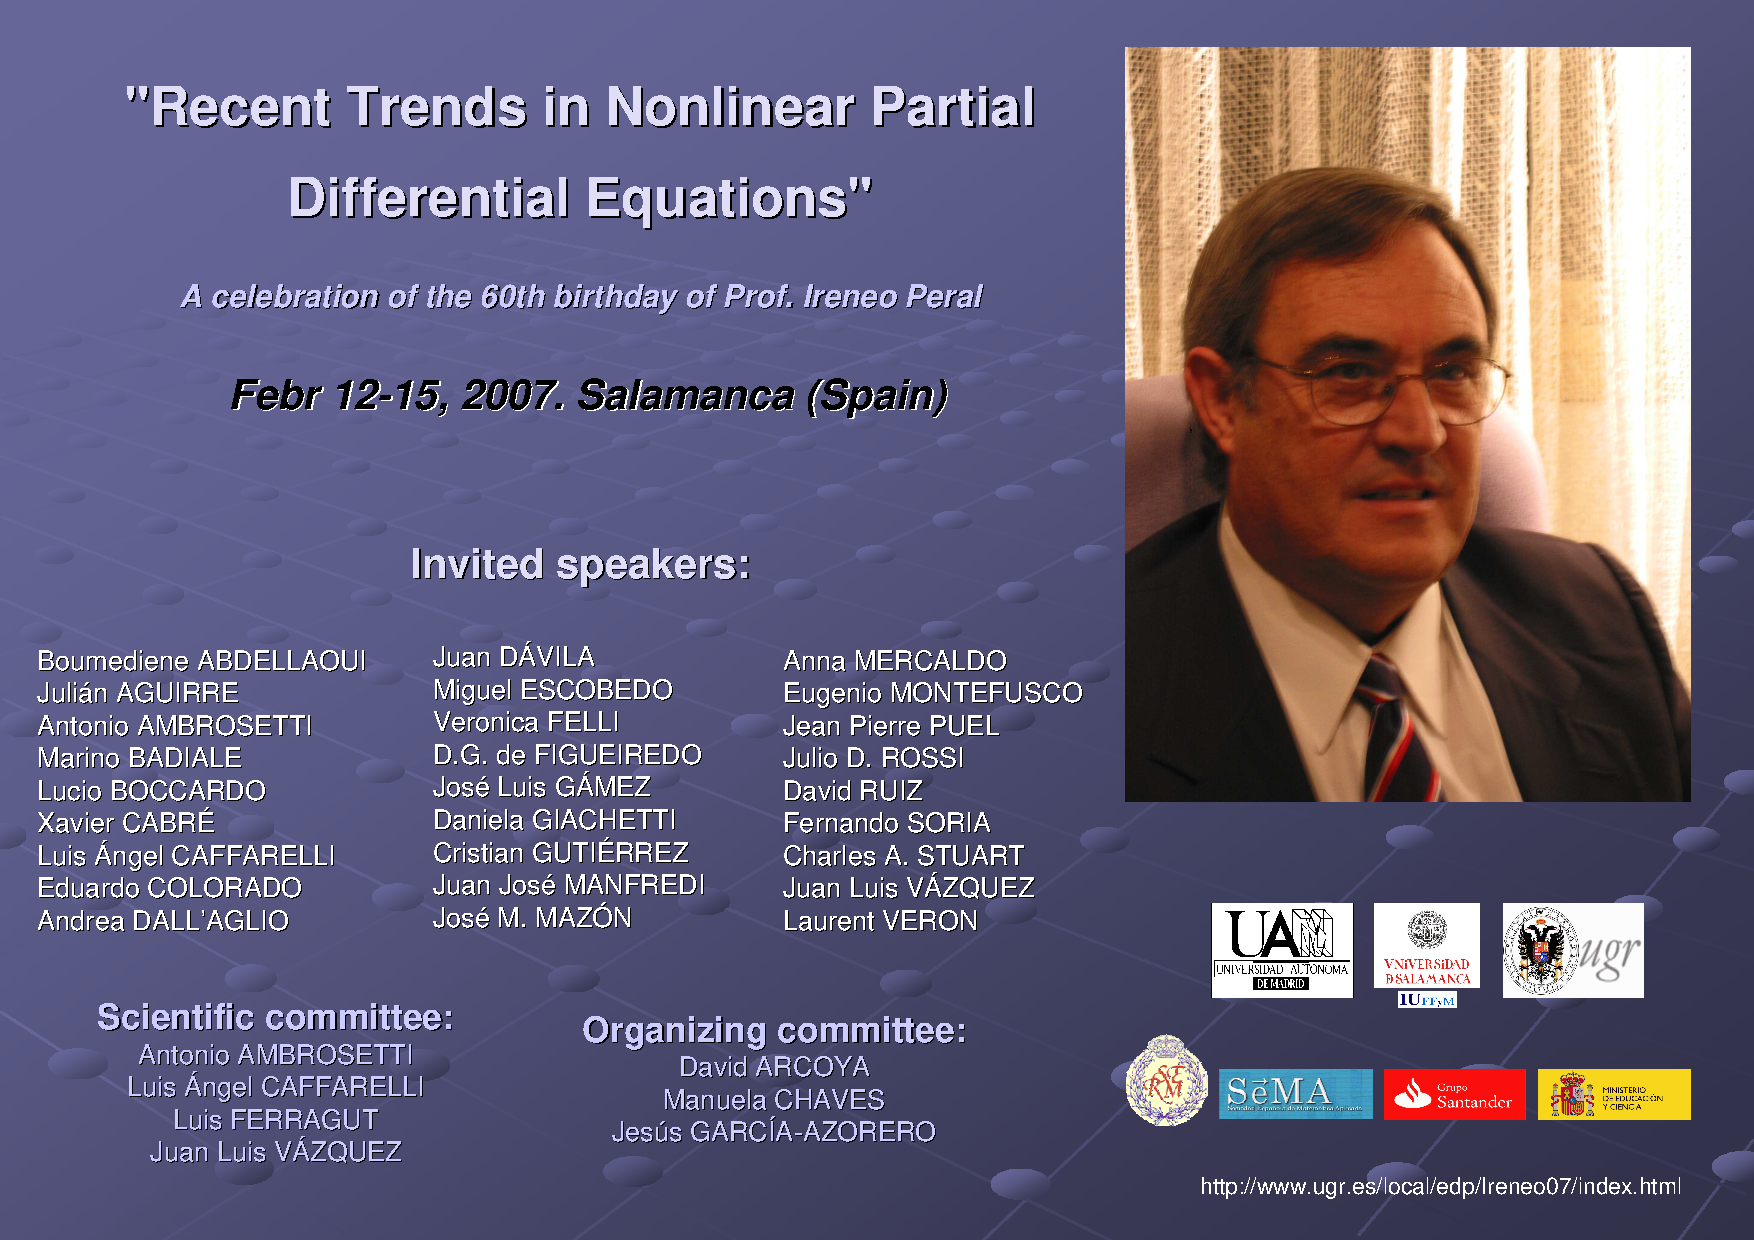
\includegraphics[width=0.9\linewidth]{IP_foto_Salamanca2007.pdf}
\caption{Cartel  del congreso en su honor celebrado en Salamanca en 2007.}
\end{center}
\end{figure}


Aparte de los trabajos con sus estudiantes de doctorado, Ireneo mantuvo colaboraciones con colegas, {algunos ya citados}, a los que siempre consider\'o amigos. De hecho, en la cena oficial de dicho Congreso de Salamanca (celebrada en el impresionante sal\'on del Colegio Fonseca) \'el mismo lo reconoci\'o con unas breves y emocionadas palabras, feliz por verse rodeado por los que consideraba sus amigos, m\'as all\'a de colegas o colaboradores. Entre todas estas colaboraciones hay dos de las que siempre se mostr\'o especialmente orgulloso. Por un lado, un art\'iculo con Juan Luis V\'azquez {(\cite{Peral-Vazquez})}, mencionado en el pre\'ambulo de su libro en De Gruyter con un agradecimiento por esta colaboraci\'on. Por otro lado, un trabajo con Luis Caffarelli {(\cite{Caffarelli-Peral})}, en el que se
obten\'ian estimaciones $W^{1,p}$ para las soluciones de familias de operadores el\'ipticos muy generales, combinando un resultado de regularidad para un operador fijo $ A_0$ con una cuidadosa comparaci\'on local entre  problemas relacionados, y finalmente  una descomposici\'on de tipo Calder\'on-Zygmund. Un bonito resultado con aplicaci\'on en problemas de homogeneizaci\'on. Ireneo siempre dec\'ia que lo m\'as estimulante era trabajar con compa\~neros que le exig\'ian salir fuera de su zona de confort matem\'atica y llegar a l\'imites para \'el inexplorados. Este trabajo con Luis Caffarelli era sin duda uno de sus favoritos.






La idea de pasar al l\'imite en problemas dependientes de un par\'ametro, en busca de comportamientos extremos, fue explorada en una direcci\'on distinta en la tesis doctoral de otro de sus estudiantes, Fernando Charro, defendida en $2009$. Juntos estudiaron c\'omo pasar al l\'imite en la familia de problemas de Dirichlet $ -\Delta_p u = \lambda u^q $ con $ q<p$, cuando $ p \to \infty $ y el resto de par\'ametros crecen de forma adecuada, con $ q/p \to Q \in (0,1) $ y $ \lambda^{1/p} \to \Lambda >0$. Con estas velocidades de convergencia, en el l\'imite encontraron soluciones viscosas de un problema completamente no lineal, $\min \{ |\nabla u|-\Lambda u^Q, - \Delta_{\infty} u \} = 0 $. Una interesante manera de combinar teor\'ia variacional con las soluciones de viscosidad, y un primer encuentro con el operador $\infty$-laplaciano, $-\Delta_{\infty} u = - \sum\limits_{i,j} u_{x_i} u_{x_j} u_{x_i x_j},$ que obligaba a salir fuera del mundo variacional, y que m\'as adelante fue uno de los muchos campos de colaboraci\'on con otro gran amigo, {Julio Rossi} {(ver por ejemplo \cite{GMPR})}. 
Gracias al apoyo de Ireneo, Fernando Charro pudo realizar 
durante su doctorado sendas estancias de investigaci\'on  en Pittsburgh  con Juanjo Manfredi y en Milan con Sandro Salsa y, una vez terminada la tesis, estancias postdoctorales  con Luis Caffarelli en Austin y con Xavier Cabr\'e en Barcelona.

Mientras se resolv\'ia su solicitud de una beca postdoctoral Fulbright-MEC con la que a la postre se marchar\'ia a EEUU con Luis Caffarelli, Ireneo le propuso a Fernando  trabajar junto con {Roberto Argiolas}, un visitante italiano reci\'en llegado, en una extensi\'on del principio del m\'aximo de Alexandroff-Bakelman-Pucci (ABP) al $p$-laplaciano. Este era un problema que ilusionaba a Ireneo y que ya hab\'ia mencionado otra veces. Sin embargo, en esa ocasi\'on, Ireneo se present\'o con una cuenta manuscrita por \'el fechada casi diez a\~nos antes donde desarrollaba una prueba extremadamente elegante de la ABP para el $p$-laplaciano en el caso de soluciones regulares. Estas ideas resultaron ser tremendamente vers\'atiles y permitieron crear un marco com\'un para probar estimaciones de tipo ABP para operadores no lineales el\'ipticos y parab\'olicos muy generales, incluyendo no solo el $p$-laplaciano sino tambi\'en los operadores de curvatura prescrita y $k$-Hessianos {(\cite{ACP})}.


En noviembre de 2007  llegaba  a Madrid Luigi Montoro, un estudiante italiano. Luigi estaba trabajando en  SISSA, Trieste, con Andrea Malchiodi en un problema el\'iptico de tipo perturbativo, con condiciones mixtas en la frontera.
	Andrea le coment\'o a Antonio Ambrosetti que Ireneo estaba interesado en el mismo tipo de problemas. Entonces, en noviembre de 2007, Ambrosetti habl\'o con Ireneo y Luigi march\'o a la UAM, donde Ireneo, amabil\'isimamente, le dio la bienvenida en italiano. Junto con Jes\'us Garc\'ia Azorero y Andrea Malchiodi estudiaron el problema perturbativo mixto {(ver \cite{GMMPI})}
	\begin{equation}\nonumber
	\begin{cases}
	-\varepsilon^2 \Delta u + u = u^p & \text{ en } \Omega; \\
	\frac{\partial u}{\partial \nu} = 0 \text{ en } \partial_{\mathcal{N}} \Omega; &
	u = 0  \text{ en } \partial_{\mathcal{D}} \Omega;
	\\ u > 0 & \text{ en } \Omega,
	\end{cases}
	\end{equation}	
	analizando la existencia de soluciones del tipo \textit{spike layers}, que se concentran en la interfaz $\mathcal{I}_\Omega$, intersecci\'on de las clausuras de los dos conjuntos, $\partial_{\mathcal{D}} \Omega$ y $\partial_{\mathcal{N}} \Omega$, en los que se divide la frontera, y estudiando tambi\'en el comportamiento y an\'alisis cualitativo de las soluciones de m\'inima energ\'ia. En palabras de Luigi, 
	\begin{quote}
	\textit{El trabajo de esta tesis estuvo siempre acompa\~{n}ado y motivado por el entusiasmo de Ireneo. \'El dec\'ia: <<la Matem\'atica es una ciencia experimental>>, es necesario probar y probar siempre. Cada d\'ia, por la tarde, cansado y feliz conclu\'ia <<Ma\~{n}ana m\'as pero no mejor, porque es imposible>>.
	El a\~no 2007 no fue solo el principio de una tesis doctoral, sino de una colaboraci\'on larga, fruct\'ifera y constante hasta el final con resultados matem\'aticos \'optimos 
y tambi\'en resultados de vida, que Ireneo ense\~{n}aba gratuitamente con amor y respeto.}
\end{quote}

\begin{figure}%[h]
\begin{center}
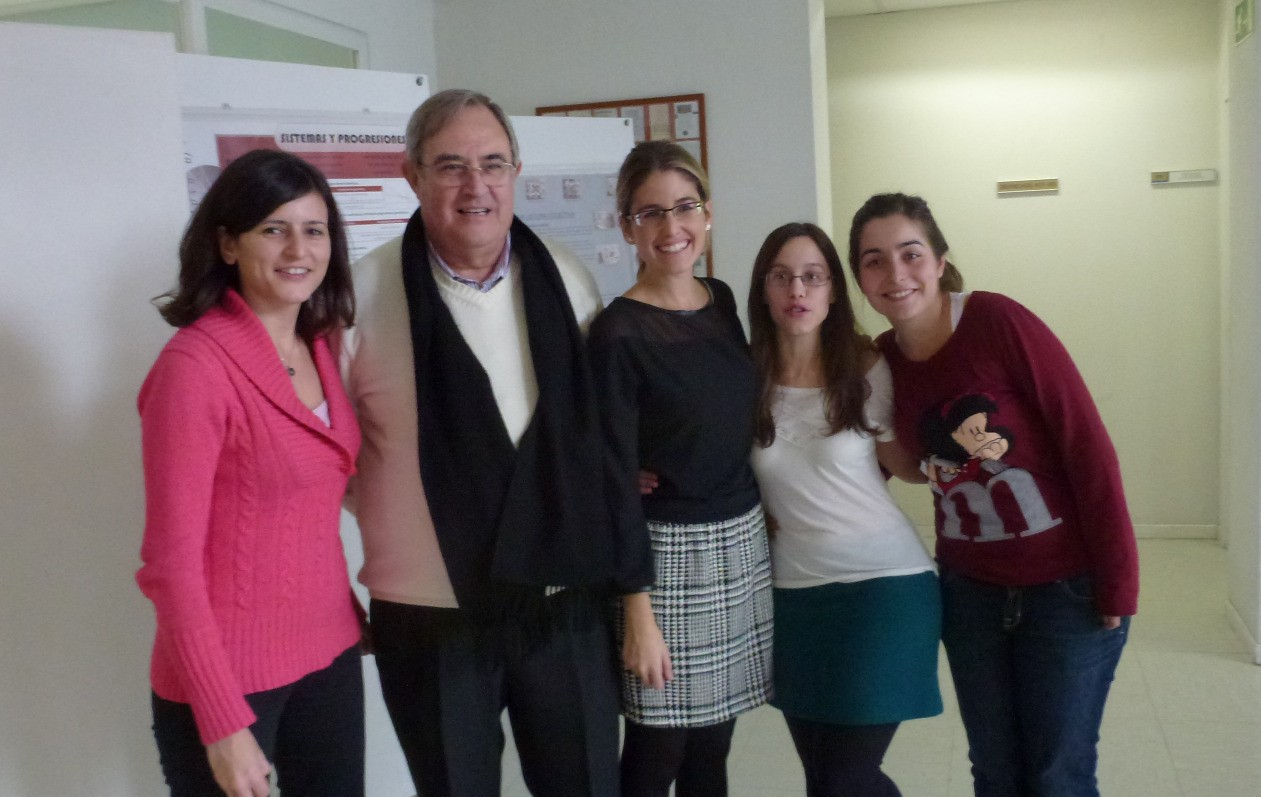
\includegraphics[width=0.9\linewidth]{IP_foto_Alumnas.jpeg}
\caption{Ireneo con sus alumnas de doctorado  A. Primo, Bego\~na Barrios, Susana Merch\'an y Mar\'ia Medina.}
\end{center}
\end{figure}
	
 
 En 2009, Ireneo incorpor\'o una estudiante m\'as, Susana Merch\'an, a trav\'es de una beca FPI de su proyecto. Susana hab\'ia hecho un Trabajo Fin de M\'aster con Ireneo sobre el problema de Kardar-Parisi-Zhang aunque el tema de su tesis gir\'o en torno a la existencia de soluciones para problemas el\'ipticos y parab\'olicos con el potencial de Hardy. Susana realiz\'o una estancia predoctoral en la Universidad de la Calabria junto a Luigi Montoro y Berardino Sciunzi que dio lugar a una fluida colaboraci\'on con este equipo de matem\'aticos {(\cite{MMPS})}. Ireneo tuvo un especial inter\'es en que sus alumnos mantuvieran una estrecha relaci\'on de trabajo, incluso terminada la tesis. De esa forma cre\'o una peque\~na escuela cuya semilla ha germinado y  se mantiene intacta hasta hoy. En ese sentido, Susana, trabaj\'o con Boumediene Abdellaoui y, junto a Ahmed Attar, produjeron varios art\'iculos de un alto nivel.

A finales de 2009 Bego\~na Barrios, que inicialmente iba a hacer su tesis en An\'alisis Arm\'onico, atra\'ida por la relaci\'on entre esta \'area y las EDP comenz\'o a estudiar bajo la direcci\'on de Fernando Soria diversos temas en el campo de los operadores no locales en un momento en el que dicha teor\'ia se expand\'ia a gran velocidad. Fernando, que hab\'ia trabajado con Luis Caffarelli y Juan Luis V\'azquez en la ecuaci\'on de los medios porosos con difusi\'on no local, le propuso a Ireneo codirigir la tesis, algo que  acept\'o de inmediato.  Ireneo, con su alegr\'ia habitual y encantado de formar parte de ello, entr\'o un d\'ia en el despacho de la que ser\'ia su nueva alumna y le dijo <<Fernando me ha hablado de ti, ma\~nana nos vemos en mi despacho y ver\'as qu\'e bien lo vamos a pasar>>. Y no se equivoc\'o. Este fue el comienzo de una fren\'etica actividad cient\'ifica por parte de Ireneo que le llev\'o a producir en un periodo de pocos a\~nos junto a sus estudiantes y colaboradores m\'as de 20 art\'iculos sobre problemas relacionados con difusi\'on no local.   

Pero volviendo a la tesis, uno de los primeros trabajos que estudi\'o Bego\~na  analizaba el problema cr\'itico 
c\'oncavo--convexo con condiciones de Dirichlet cero para el laplaciano fraccionario espectral $A_{s}u(x):=\sum
  \rho_j^{s}a_j\varphi_j(x),\quad x\in \Omega,$
siendo $u(x)=\sum a_j\varphi_j(x)$, $x\in\Omega$ y $(\varphi_j,\rho_j)$ las autofunciones y autovalores del laplaciano $(-\Delta)$ en $\Omega$ con condiciones Dirichlet cero. Este resultado  motivar\'ia el estudio del mismo problema para el operador definido como integral singular unos a\~nos m\'as tarde. El siguiente, desarrollado en gran parte durante la estancia predoctoral de Bego\~na Barrios en la Universit\`a degli Studi di Milano Statale  con Enrico Valdinocci, vers\'o sobre un argumento de regularidad tipo bootstrap para operadores integro-diferenciales generales 
$$Iu(x)= \frac{1}{2}\int_{\mathbb R^N} (u(x+y) + u(x-y) - 2u(x)) K(x,y)\, dy,$$
que posteriormente se aplic\'o para obtener la regularidad $\mathcal{C}^{\infty}$ de las superficies m\'inimas no locales en un trabajo conjunto con Figalli y Valdinoci. Este \'ultimo trabajo, a su vez, permiti\'o a Bego\~na trabajar con estos dos expertos en el \'area y establecer una relaci\'on matem\'atica y personal que dio lugar a visitas del profesor {Valdinocci} y de algunos de sus colaboradores a la UAM, creando as\'i momentos de charlas de pizarra en el despacho de Ireneo y el inicio de otras colaboraciones como la del estudio del Teorema de Widder para la ecuaci\'on del calor fraccionaria, problema que a \'el  le apasionaba {(\cite{BPSV})}. Asimismo estas colaboraciones internacionales fueron el impulso para que, tiempo despu\'es, Bego\~na realizara su primer postdoctorado bajo la direcci\'on de Alessio Figalli en la Universidad de Austin. 

No todos los trabajos de Ireneo de esta \'epoca est\'an relacionados con  difusi\'on fraccionaria. En este periodo mantiene una intensa colaboraci\'on con Carlos Escudero sobre diversos problemas de la F\'isica relacionados con crecimiento epitaxial as\'i como sobre ecuaciones en derivadas parciales de cuarto orden conjuntamente, entre otros, con  Fillipo Gazzola.
	
En noviembre de 2011 comenzaba su doctorado la que ser\'ia la \'ultima estudiante de Ireneo, Mar\'ia Medina. Aunque inicialmente esta tesis iba a girar en torno a los operadores de cuarto orden y su interacci\'on con diversas no linealidades, el auge de los fen\'omenos no locales hizo a Ireneo proponer un cambio en la tem\'atica del trabajo. De la mano de Bego\~na Barrios, que a\'un era estudiante, ambas comenzaron a estudiar el efecto del potencial de Hardy fraccionario en problemas con el laplaciano fraccionario como operador principal. Esta colaboraci\'on culmin\'o en dos trabajos, uno  en el que se revisitaba el cl\'asico problema c\'oncavo-convexo en este marco no local, 
y un segundo donde se consideran t\'erminos singulares en la frontera, teniendo as\'i ecuaciones doblemente singulares. El siguiente paso consisti\'o en estudiar la regularidad de las soluciones de estos problemas con el potencial de Hardy no local en funci\'on de la regularidad de los datos. Este an\'alisis deriv\'o a su vez en otros dos trabajos, uno el\'iptico y otro parab\'olico, en colaboraci\'on con  Boumediene Abdellaoui y Ana Primo.

Ha quedado claro que para Ireneo la movilidad internacional era fundamental en la formaci\'on de sus estudiantes. No lo fue menos en el caso de Mar\'ia Medina. As\'i, a lo largo de su tesis Mar\'ia llev\'o a cabo  estancias de formaci\'on, primero en la University of Pittsburgh, bajo la supervisi\'on de Juan J. Manfredi, y luego en el Weierstrass Institute for Applied Analysis and Stochastics (WIAS) de Berl\'in. En esta \'ultima, ya en tercer a\~no de doctorado, Mar\'ia tuvo la oportunidad de colaborar con {Enrico Valdinoci y Serena Dipierro} y comenzar a estudiar los llamados fen\'omenos de concentraci\'on y los m\'etodos de reducci\'on finito-dimensional {(\cite{DMPV})}. Este trabajo supuso el final de la tesis de Mar\'ia, pero el inicio del que ser\'ia el tema principal de su investigaci\'on posdoctoral. 

 Como ha quedado reflejado en lo que a la recopilaci\'on  de los trabajos de sus alumnos se refiere, la direcci\'on de tesis ocup\'o gran parte de la vida acad\'emica de Ireneo. Se involucr\'o en ello, tanto en lo profesional como en lo personal, como pocos lo han hecho. Sus alumnos terminaban sus tesis con un importante bagaje de art\'iculos bajo el brazo. Pero tambi\'en con la sensaci\'on de pertenecer a una familia, la de Ireneo y Magdalena, que les recib\'ia con los brazos abiertos, les ayudaba con sus necesidades del d\'ia a d\'ia, especialmente a los que no eran de Madrid,  celebraba con ellos sus alegr\'ias y les animaba en sus penas, cuando alguna vez las padecieron. Ireneo siempre estaba disponible para ellos y para cualquier otro invitado que llegara al departamento. Cre\'ia y defend\'ia la universidad p\'ublica de calidad y puso de su parte, {como investigador, docente y gestor},  todo lo que estuvo en su mano para lograr que la suya lo fuera. Un d\'ia calcul\'o la distancia que hab\'ia recorrido yendo al departamento en sus m\'as de 40 a\~nos de servicio en la Universidad Aut\'onoma de Madrid: le salieron cerca de 250.000 kil\'ometros. Cuando se jubil\'o, como pofesor em\'erito sigui\'o a\~nadiendo a estos unos pocos m\'as. Tiene raz\'on Borges, \textit{\lq esas\rq\, personas est\'an salvando el mundo.}
 
\begin{thebibliography}{99} %\textsc
\small
\bibitem{ADP}    \textsc{B. Abdellaoui, A. Dall'Aglio, I. Peral,} Some remarks on elliptic problems with critical growth in the gradient,  \textit{J. Differential Equations} \textbf{222} (2006), no.1, 21--62.
 
\bibitem{AP2}    \textsc{B. Abdellaoui, I. Peral,} Existence and nonexistence results for quasilinear elliptic equations involving the p-Laplacian with a critical potential,  \textit{Ann. Mat. Pura Appl.}  \textbf{182} (2003), no.3, 247--270.

 \bibitem{APP}   \textsc{B. Abdellaoui, I. Peral, A. Primo}, {Elliptic problems with a Hardy potential and critical growth in the gradient: non-resonance and blow-up results.} \textit{J. Differential Equations} \textbf{239} (2007), no. 2, 386--416.

 \bibitem{APP1}    \textsc{B. Abdellaoui, I. Peral, A. Primo}, {Breaking of resonance and regularizing effect of a first order quasi-linear term in some elliptic equations}, \textit{Annales de l'Institut Henri Poincare} \textbf{25} (2008), no. 5,  962--985.

\bibitem{APP3}    \textsc{B. Abdellaoui, I. Peral, A. Primo}, {Optimal results for parabolic problems arising in some physical models with critical growth in the gradient respect to a Hardy potential}. \textit{Adv. Math.} \textbf{225} (2010), no. 6,  2967--3021.

\bibitem{Aguilar-Peral_5}    \textsc{J.A. Aguilar, I. Peral,} Global behaviour of the Cauchy Problem for some Critical Nonlinear Parabolic Equations, \textit{SIAM Journal in Mathematical Analysis} \textbf{31}  (2000), no. 6, 1270--1294. 


\bibitem{Aguirre-Peral}   \textsc{J. Aguirre, I. Peral,} Existence of periodic solutions for a class of nonlinear equations,\textit{Contributions to nonlinear partial differential equations (Madrid, 1981)}, 1--6,  Res. Notes in Math. \textbf{89}, Pitman, Boston, MA, 1983.


 \bibitem{AGP}    \textsc{A. Ambrosetti, J. Garc\'ia Azorero, I. Peral,}  Multiplicity of solutions for semilinear and quasilinear elliptic problems. \textit{J. Funct. Anal.} \textbf{137} (1996),  219--242.

\bibitem{Ambrosetti-Peral_1}    \textsc{A. Ambrosetti,  J. Garc\'ia Azorero, I. Peral,} Perturbation of $-\Delta u + u^{(N+2)/(N-2)} = 0$, the scalar curvature problem in $\mathbb{R}^N$ and related topics, \textit{J. Funct. Anal.} \textbf{165} (1999),  no. 1,  117--149. 


\bibitem{Ambrosetti-Peral_2}    \textsc{A. Ambrosetti,  J. Garc\'ia Azorero, I. Peral,} Elliptic variational problems in $\mathbb{R}^N$ with critical growth, \textit{J. Differential Equations} \textbf{168}  (2000), no. 1, 10--32. 

\bibitem{Ambrosetti-Peral_3}    \textsc{A. Ambrosetti,  J. Garc\'ia Azorero, I. Peral,} Existence and Multiplicity Results for Some Nonlinear Elliptic Equations: A Survey, \textit{Rendiconti di Matematica Univ. Roma}, Seria VII Vol. 20 (in Honor to G. Fichera) (2000), 167--198.

\bibitem{Ambrosetti-Peral_4}    \textsc{A. Ambrosetti,  J. Garc\'ia Azorero, I. Peral,} Remarks on a class of Semilinear Elliptic equations on $\mathbb{R}^n$, via perturbation Methods, \textit{Adv. Nonlinear Studies} \textbf{1} (2001), 1--15.

\bibitem{AP}  \textsc{D. Arcoya, I. Peral,} En recuerdo de un maestro y amigo, Antonio Ambrosetti.  \textit{Gac. R. Soc. Mat. Esp.} \textbf{24} (2021), no. 1, 25--34

\bibitem{ACP}    \textsc{R. Argiolas, F. Charro,   and I. Peral}, {On the Aleksandrov-Bakel'man-Pucci estimate for some elliptic and parabolic nonlinear operators}, \textit{Arch. Ration. Mech. Anal.} \textbf{202} (2011), no. 3, 875--917.

\bibitem{BPSV}    \textsc{B. Barrios, I. Peral, F. Soria, E. Valdinoci},  A Widder's type Theorem for the heat equation with nonlocal diffusion. \textit{Arch. Ration. Mech. Anal.} \textbf{213} (2014) no. 2, 629--650. 
 
\bibitem{Boccardo-Escobedo-Peral}    \textsc{L. Boccardo, M. Escobedo, I. Peral},  A remark on Elliptic Problems involving critical exponent. \textit{Nonlinear Analysis T.M.A.} \textbf{24}  (1995), no. 11, 1639--1648.

 \bibitem{BOP}    \textsc{L. Boccardo, L. Orsina, I. Peral},  A remark on existence and optimal summability of solutions of elliptic problems involving Hardy potential. \textit{Discrete Contin. Dyn. Syst.} \textbf{16} (2006), no. 3, 513--523. 

\bibitem{Caffarelli-Peral}    \textsc{L. A. Caffarelli, I. Peral,} On $ W^{1,p}$ estimates for elliptic equations, \textit{Comm. in Pure Appl. Math.} \textbf{51} (1998),  1--21.

 \bibitem{Col-Per2}    \textsc{E. Colorado, I.  Peral, } Eigenvalues and bifurcation for elliptic equations with mixed Dirichlet-Neumann boundary conditions related to Caffarelli-Kohn-Nirenberg inequalities. \textit{Topol. Methods Nonlinear Anal.} \textbf{23} (2004), no. 2, 239--273.

\bibitem{DMPV}    \textsc{S. Dipierro, M. Medina, I. Peral, E. Valdinoci}, Bifurcation results for a fractional elliptic equation with critical exponent in $\mathbb{R}^n$, \textit{Manuscripta Mathematica} \textbf{153} (2017), no. 1, 183--230.
 
\bibitem{GMMPI}    \textsc{J. Garc\'{i}a Azorero, A. Malchiodi,  L. Montoro, I.  Peral},  Concentration of solutions for some singularly perturbed
mixed problems: existence results. \textit{Arch. Ration. Mech. Anal.} \textbf{196} (2010), no. 3, 907--950.
 
\bibitem{Azorero-Manfredi-Peral}    \textsc{J. Garc\'ia Azorero, J.J. Manfredi, I. Peral,} Sobolev versus H\"older Minimizers with Applications to Quasilinear Elliptic Equations, \textit{Comm. in Contemporary Math.} \textbf{2}  (2000), no. 3,  385--404.

\bibitem{GMPR}    \textsc{J. Garcia Azorero, J.J. Manfredi, I Peral, J. Rossi},  D. Limits for Monge-Kantorovich mass transport problems. \textit{Comm. Pure Appl. Anal.} \textbf{7} (2008), no. 4, 853--865.

\bibitem{Azorero-Peral_1}    \textsc{J. Garc\'ia Azorero, I. Peral,} Existence and nonuniqueness for the p-laplacian: Nonlinear eigenvalues, \textit{Comm. in Partial Differential Equations} \textbf{12}  (1987), no. 12,  1389--1430. 

\bibitem{Azorero-Peral_4}   \textsc{J.Garc\'ia Azorero, I. Peral,} Multiplicity of solutions for elliptic problems with critical exponents or with a non-symmetric term. \textit{Trans. Amer. Math. Soc.} \textbf{323} (1991), no. 2, 877--895. 

\bibitem{Azorero-Peral_5}   \textsc{J. Garc\'ia Azorero, I. Peral Alonso},  Hardy inequalities and some critical elliptic and parabolic problems. \textit{J. Differential Equations} \textbf{144} (1998), no. 2, 441--476.

\bibitem{MMPS}   \textsc{S. Merch\'an, L. Montoro,  I. Peral, B. Sciunzi, }, {Existence and qualitative properties of solutions to  a quasilinear elliptic equation involving the Hardy-Leray potential}, \textit{Ann. Inst. H. Poincar\'e Anal. Non Lin\'eaire} \textbf{31} (2014), no. 1, 1--22.

 \bibitem{IP1}  \textsc{I. Peral Alonso} Entrevista a Yves Meyer, Premio Abel 2017, un excepcional matem\'atico, itinerante y visionario. \textit{Gac. R. Soc. Mat. Esp.} \textbf{20} (2017), no. 3, 493--512
  
\bibitem{PSbook}    \textsc{I. Peral, F. Soria}, \textit{Elliptic and Parabolic Equations Involving the Hardy-Leray Potential}, De Gruyter Series in Nonlinear Analysis and Applications \textbf{38}, 2021.
 
\bibitem{Peral-Vazquez}    \textsc{I. Peral, J.L. Vazquez,} On the Stability or Instability of the Singular Solution of the Semilinear Heat Equation with Exponential Reaction Term. \textit{Arch. Ration. Mech. Anal.} 
\textbf{129} (1995),  no. 3, 201--224.

\normalsize
\begin{center}
%\mbox{}\\[.1ex]
\resizebox{.5\linewidth}{!}{\color{azulsema}\rule{.5\linewidth}{1pt}
{\large $\diamond$} {\huge $\diamond$} {\large $\diamond$} \rule{.5\linewidth}{1pt}}
\end{center}
\end{thebibliography}

%\printcontact
%
%\endinput
%
%%---------------------------


